\documentclass[a4paper,14pt]{extarticle}

\usepackage[a4paper,top=20mm,bottom=20mm,left=30mm,right=10mm]{geometry}
\usepackage[T1,T2A]{fontenc}
\usepackage[utf8]{inputenc}
\usepackage[russian]{babel}
\usepackage{indentfirst}
\usepackage{titlesec}
\usepackage{graphicx}
\usepackage{listings}

\renewcommand{\baselinestretch}{1.3}
\titleformat{\section}{\normalsize\bfseries}{\thesection}{1em}{}
\titleformat{\subsection}{\normalsize\bfseries}{\thesection}{1em}{}
\setlength{\parindent}{12.5mm}

\begin{document}
	
	\newpage\thispagestyle{empty}
	\begin{center}
		\MakeUppercase{
			Министерство науки и высшего образования Российской Федерации\\
			Федеральное государственное бюджетное образовательное учреждение высшего образования\\
			<<Вятский Государственный Университет>>\\
		}
		Институт математики и информационных систем\\
		Факультет автоматики и вычислительной техники\\
		Кафедра электронных вычислительных машин
	\end{center}
	\vfill
	
	\begin{center}
		Отчет по лабораторной работе №3\\
		по дисциплине\\
		<<Информатика>>\\
		<<Реализация базовых алгоритмов в системах счисления>>
	\end{center}
	\vfill
	
	\noindent
	\begin{tabular}{ll}
		Выполнил студент гр. ИВТб-1301-05-00 \hspace{5mm} &
		\rule[-1mm]{25mm}{0.10mm}\,/Макаров С.А./\\
		
		Руководитель доцент кафедры ЭВМ & \rule[-1mm]{25mm}{0.10mm}\,/Коржавина А.С./\\
	\end{tabular}
	
	\vfill
	\begin{center}
		Киров 2024
	\end{center}
	
	\newpage
	\section*{Цель}
	Цель лабораторной работы: закрепить на практике лекционный материал по теме «Системы счисления», реализовав несколько базовых алгоритмов работы в системах счисления с произвольными основаниями.
	
	\section*{Задание}
	\begin{enumerate}
		\item Определить количество нулей в двоичной записи числа. На входе: целое неотрицательное число в десятичной системе счисления. На выходе: количество нулей в двоичной записи числа.
		
		\item Определить, какая цифра, 0 или 1, стоит в разряде N в двоичной записи числа. На входе: через пробел целое неотрицательное число в десятичной системе счисления, номер разряда в двоичной записи числа. На выходе: двоичная цифра в разряде номер N.
		
		\item Перевести вещественное число X из системы счисления с основанием K. Перевести число в систему счисления с основанием M. На входе: в одну строку через пробел 3 числа: вещественное число X, Целое число K из диапазона 2..10, целое число M из диапазона 2..10. На выходе: вещественное число в системе счисления с основанием M. Количество знаков дробной части определять исходя из количества знаков исходного числа.
	\end{enumerate}
	
	\newpage
	\section*{Решение}
	\subsection*{Задание 1}
	Схема алгоритма для решения предлагаемой задачи представлена на рисунке 1.
	
	\begin{figure}[h]
		\centering
		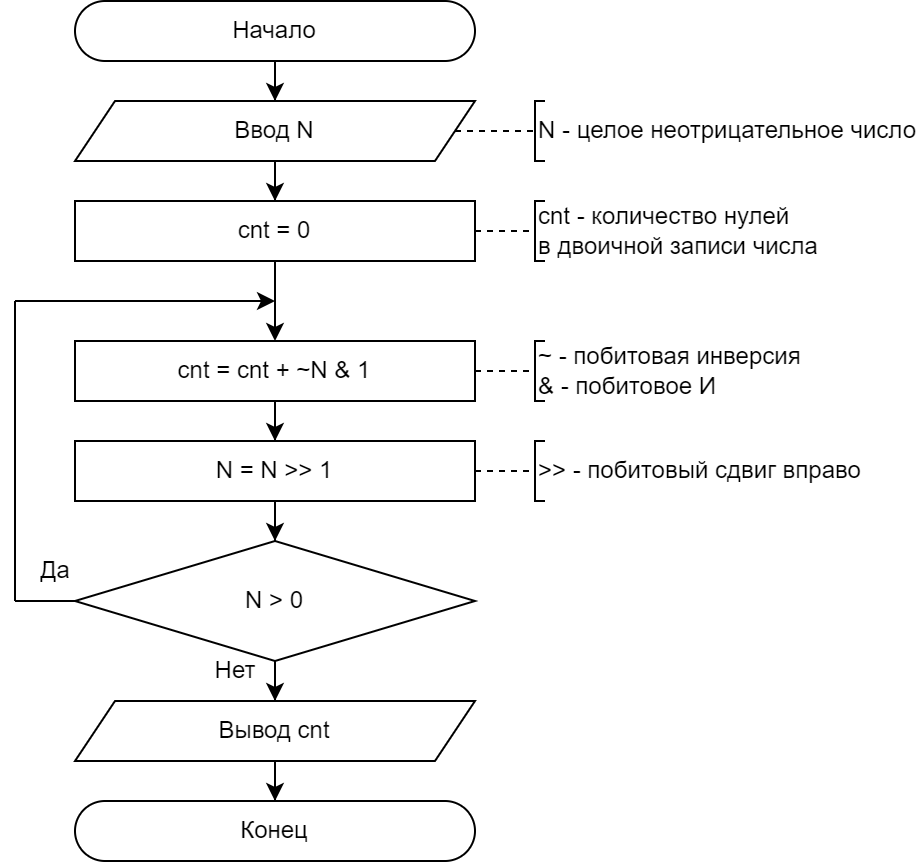
\includegraphics[width=0.68\linewidth]{schemes/s-1}
	\end{figure}
	\begin{center}
		Рисунок 1 – Схема алгоритма задания 1
	\end{center}
	
	Решение задачи на языке C представлено ниже.
	
	\begin{lstlisting}[tabsize=2,basicstyle=\ttfamily]
#include <stdio.h>
int main() {
	int N, cnt = 0;
	scanf("%d", &N);
	do {
		cnt += ~N & 1, N >>= 1;
	} while (N);
	printf("%d", cnt);
	return 0;
}
	\end{lstlisting}
	
	\subsection*{Задание 2}
	Схема алгоритма для решения предлагаемой задачи представлена на рисунке 2.
	
	\begin{figure}[h]
		\centering
		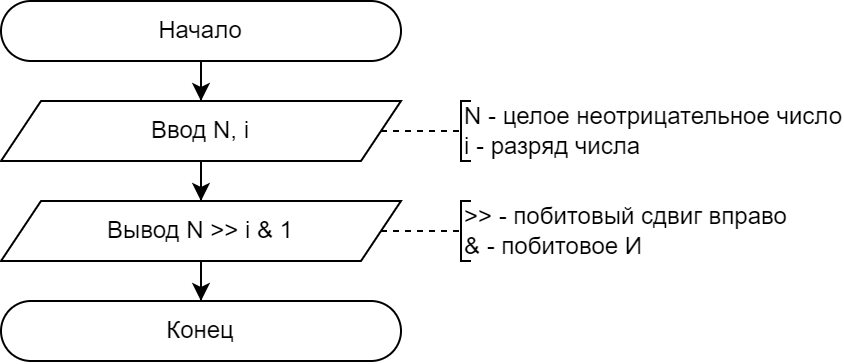
\includegraphics[width=0.68\linewidth]{schemes/s-2}
	\end{figure}
	\begin{center}
		Рисунок 2 – Схема алгоритма задания 2
	\end{center}
	
	Решение задачи на языке C представлено ниже.
	
	\begin{lstlisting}[tabsize=2,basicstyle=\ttfamily]
#include <stdio.h>
int main() {
	int N, i;
	scanf("%d %d", &N, &i);
	printf("%d", N >> i & 1);
	return 0;
}
	\end{lstlisting}
	
	\newpage
	\subsection*{Задание 3}
	Схема алгоритма для решения предлагаемой задачи представлена на рисунке 3.1. Схемы подпрограмм <<Разделение числа>> и <<Количество символов>> представлены на рисунках 3.2 и 3.3 соответственно. Также использовались подпрограммы <<Перевод в 10 СС>> и <<Перевод в M СС>>, схемы которых изображены на рисунках 3.4 и 3.5 соответственно.
	
	\begin{figure}[h]
		\centering
		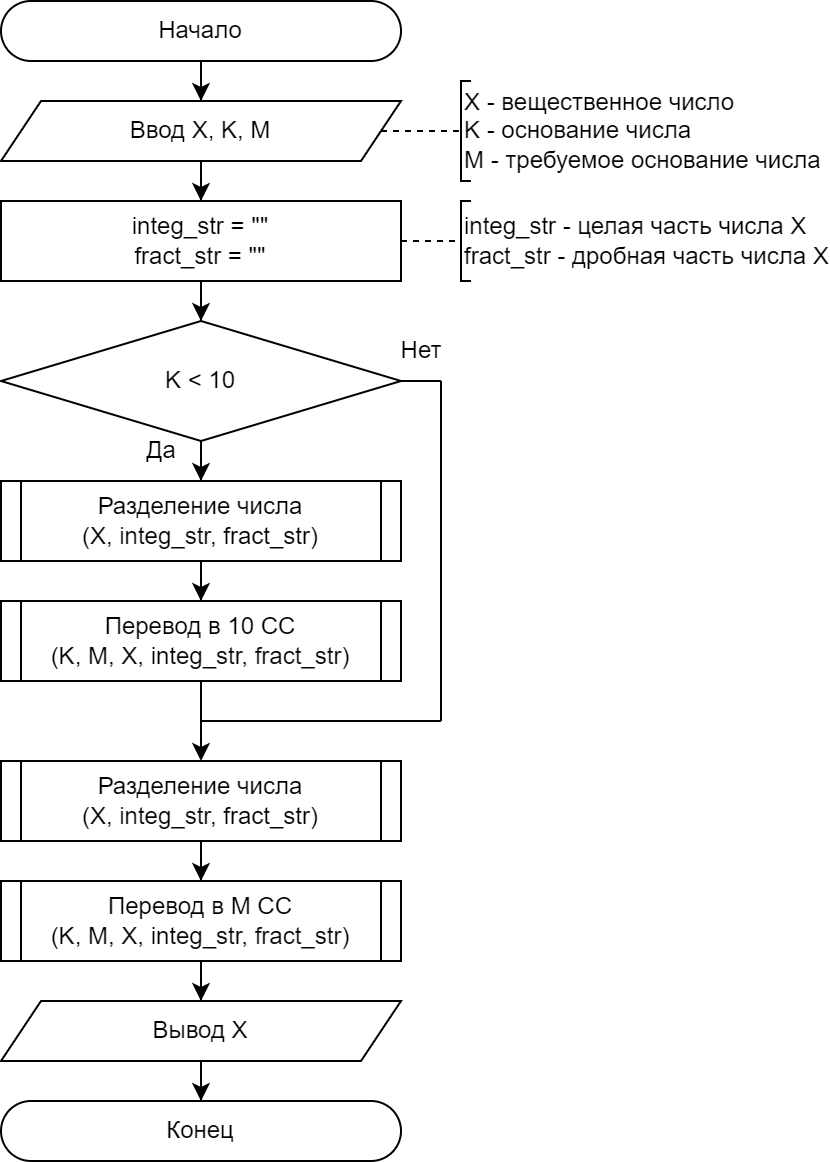
\includegraphics[width=0.6\linewidth]{schemes/s-3-1}
	\end{figure}
	\begin{center}
		Рисунок 3.1 – Схема алгоритма задания 3
	\end{center}
	\pagebreak
	
	\begin{figure}[h]
		\centering
		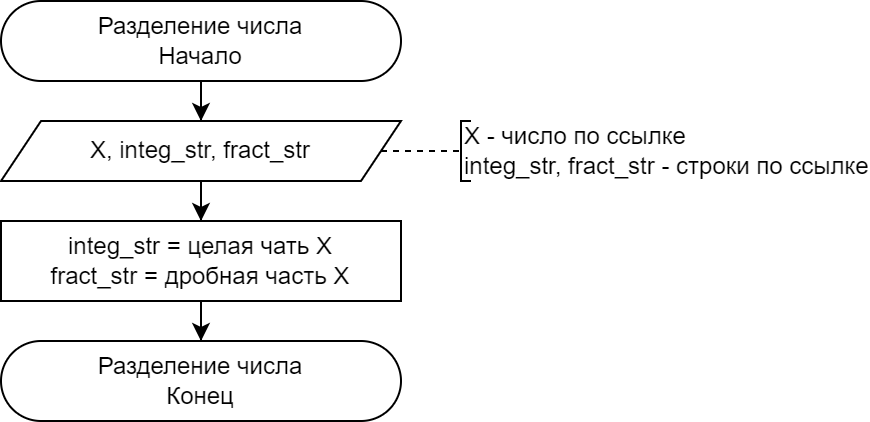
\includegraphics[width=0.6\linewidth]{schemes/s-3-2}
	\end{figure}
	\begin{center}
		Рисунок 3.2 – Схема алгоритма подпрограммы <<Разделение числа>>
	\end{center}
	
	\begin{figure}[h]
		\centering
		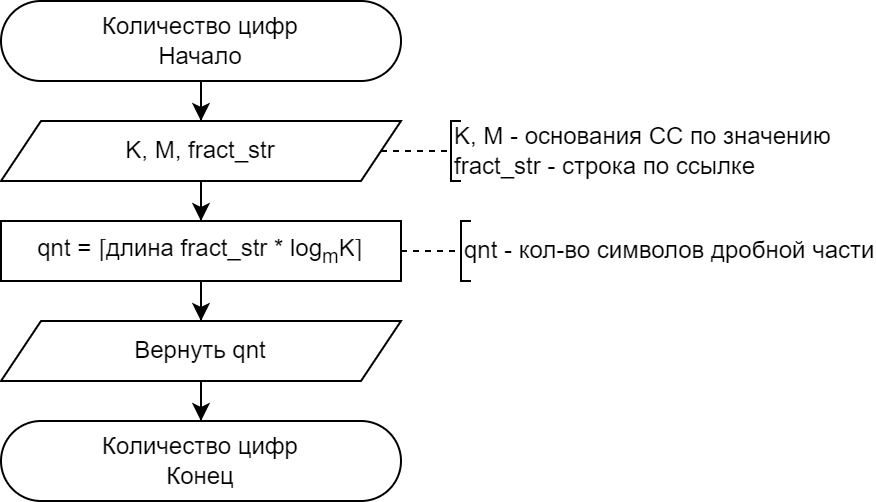
\includegraphics[width=0.6\linewidth]{schemes/s-3-3}
	\end{figure}
	\begin{center}
		Рисунок 3.3 – Схема алгоритма подпрограммы <<Количество символов>>
	\end{center}
	\pagebreak
	
	\begin{figure}[h]
		\centering
		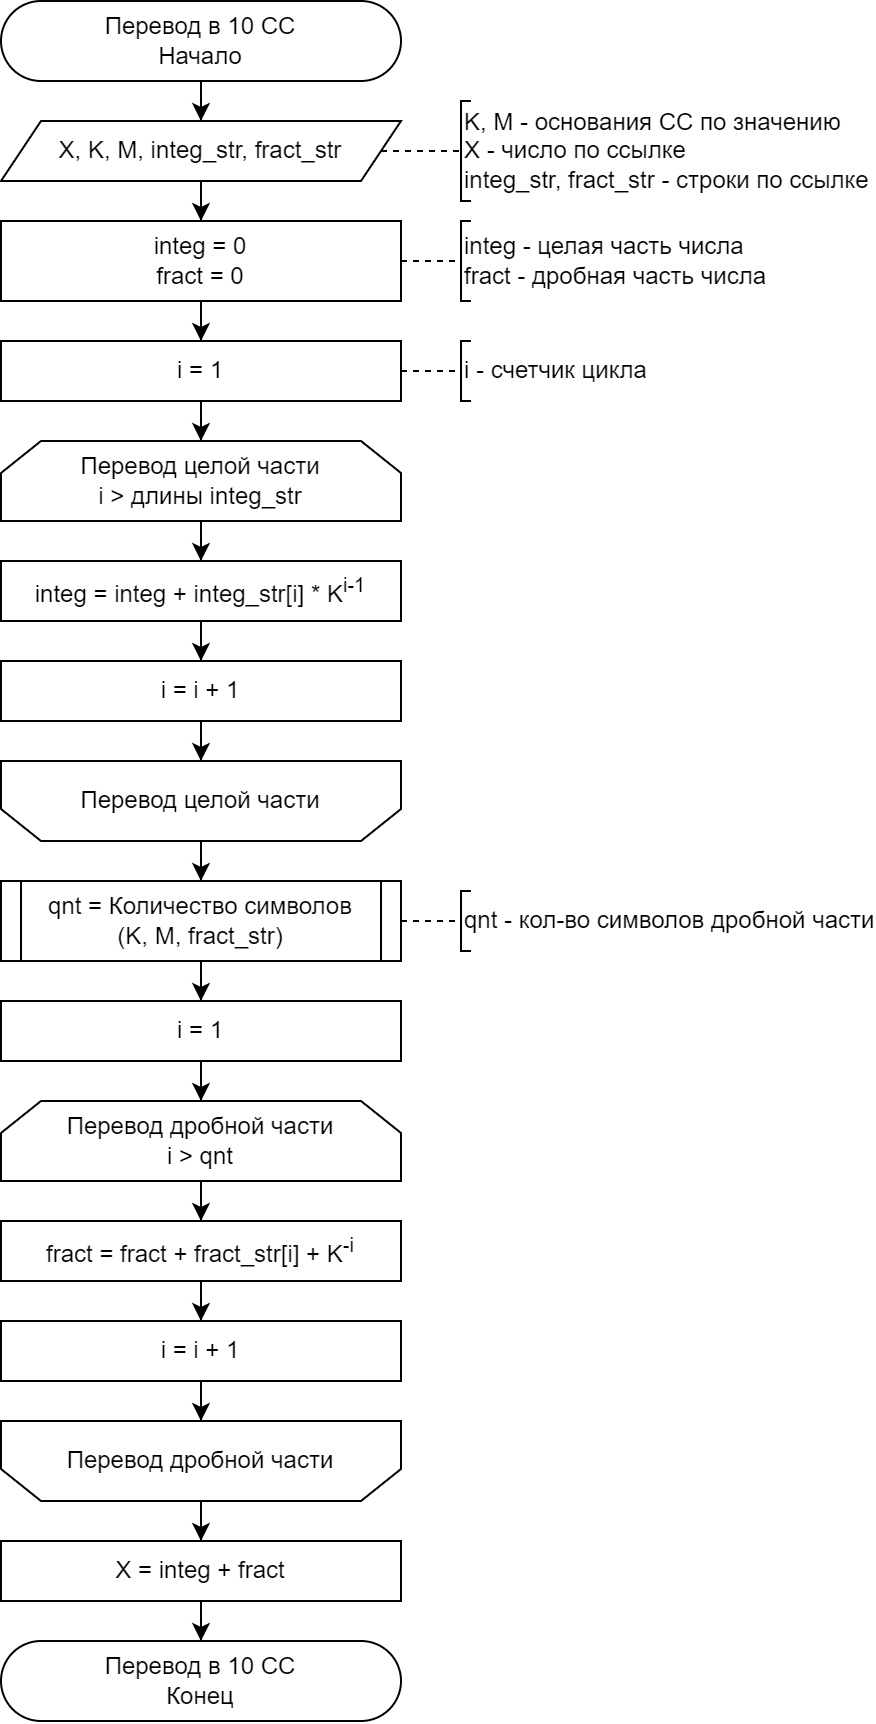
\includegraphics[width=0.59\linewidth]{schemes/s-3-4}
	\end{figure}
	\begin{center}
		Рисунок 3.4 – Схема алгоритма подпрограммы <<Перевод в 10 СС>>
	\end{center}
	\pagebreak
	
	\begin{figure}[h]
		\centering
		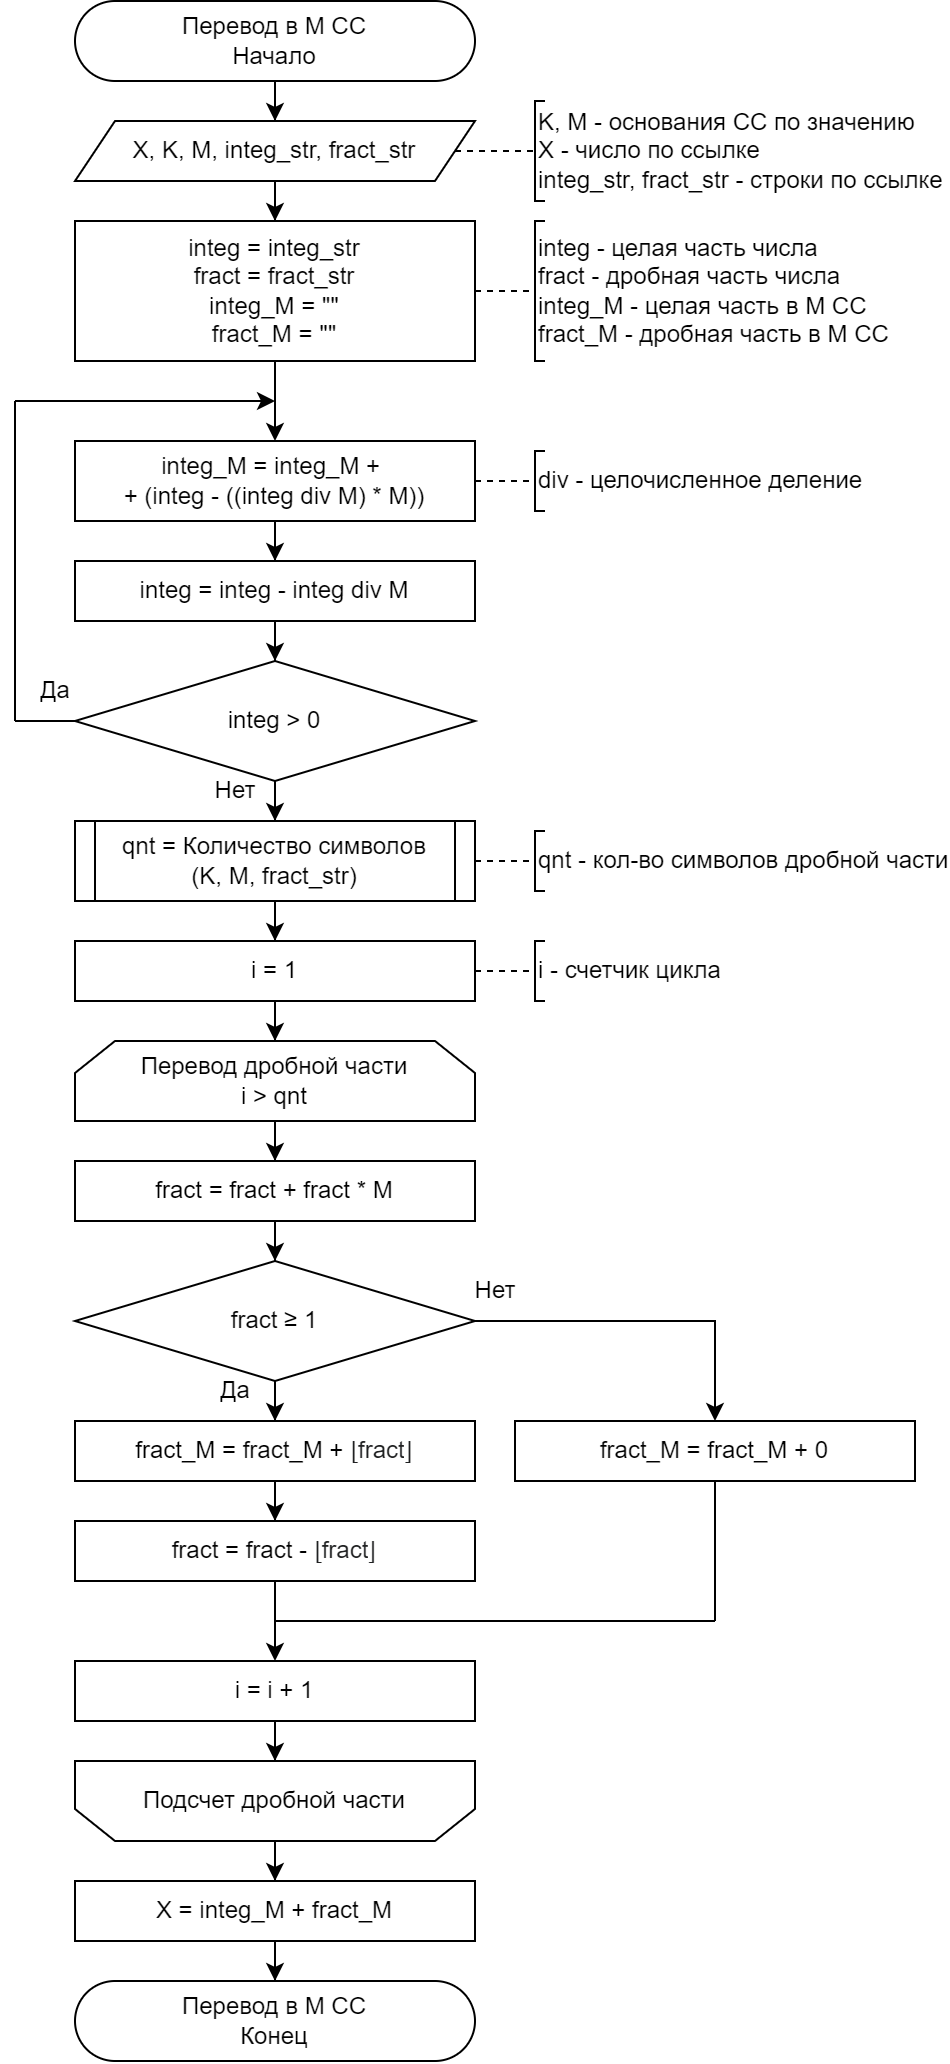
\includegraphics[width=0.54\linewidth]{schemes/s-3-5}
	\end{figure}
	\begin{center}
		Рисунок 3.5 – Схема алгоритма подпрограммы <<Перевод в M СС>>
	\end{center}
	\pagebreak
	
	Решение задачи на языке C представлено ниже.
	
	\begin{lstlisting}[tabsize=2,basicstyle=\ttfamily]
#include <stdio.h>
#include <stdlib.h>
#include <string.h>
#include <math.h>
int quantity(int K, int M, char *fract_str) {
	return ceil(strlen(fract_str) * (log(K) / log(M)));
}
void divide_num(char *X, char *integ_str, 
								char *fract_str) {
	sprintf(integ_str, "%s", strtok(X, "."));
	sprintf(fract_str, "%s", strtok(NULL, "."));
}
void translate_to_10(int K, int M, char *X, 
							char *integ_str, char *fract_str) {
	int integ_sum = 0; float fract_sum = 0;
	for (int i = 0; i < strlen(integ_str); i++) {
		integ_sum += (integ_str[i] - '0') 
								* pow(K, strlen(integ_str) - i - 1);
	}
	for (int i = 0; i < quantity(K, M, fract_str); i++) {
		fract_sum += (fract_str[i] - '0') 
								* (1 / pow(K, i + 1));
	}
	sprintf(X, "%g", integ_sum + fract_sum);
}
void translate_to_M(int K, int M, char *X, 
							char *integ_str, char *fract_str) {
	char integ_M[32], fract_M[32] = "", bf[32] = "0.";
	itoa(atoi(integ_str), integ_M, M);
	strcat(bf, fract_str);
	float fract = atof(bf);
	for (int i = 0; i < quantity(K, M, fract_str); i++) {
		fract *= M;
		if (fract >= 0) {
			char bf[2];
			itoa((int)floor(fract), bf, 10);
			strcat(fract_M, bf);
			fract -= floor(fract);
		} else {
			strcat(fract_M, "0");
		}
	}
	sprintf(X, "%s", integ_M);
	strcat(X, "."); strcat(X, fract_M);
}
int main() {
	char X[32]; int K, M; 
	char integ_str[16], fract_str[16];
	scanf("%s %d %d", X, &K, &M);
	if (K < 10) {
		divide_num(X, integ_str, fract_str);
		translate_to_10(K, M, X, integ_str, fract_str);
	}
	divide_num(X, integ_str, fract_str);
	translate_to_M(K, M, X, integ_str, fract_str);
	printf("%s", X);
	return 0;
}
	\end{lstlisting}
	
	\section*{Вывод}
	В ходе выполнения лабораторной работы удалось закрепить на практике знания использования различных систем счисления, реализовав алгоритмы работы с целыми и вещественными числами в различных системах счисления.
	
\end{document}